
% Many thanks to Andrew West for writing most of this file
% Main LaTeX file for CIS400/401 Project Proposal Specification
%
% Once built and in PDF form this document outlines the format of a
% project proposal. However, in raw (.tex) form, we also try to
% comment on some basic LaTeX technique. This is not intended to be a
% LaTeX tutorial, instead just (1) a use-case thereof, and (2) a
% template for your own writing.

% Ordinarily we'd begin by specifying some broad document properties
% like font-size, page-size, margins, etc. -- We have done this (and
% much more) for you by creating a 'style file', which the
% 'documentclass' command references.
\documentclass{sig-alternate}
 
% These 'usepackage' commands are a way of importing additional LaTeX
% styles and formattings that aren't part of the 'standard library'
\usepackage{mdwlist}
\usepackage{url}

\begin{document} 
\nocite{*}
% We setup the parameters to our title header before 'making' it. Note
% that your proposals should have actual titles, not the generic one
% we have here.
\title{Electronic Knee Wrap for Injury Prediction}
\subtitle{Dept. of CIS - Senior Design 2013-2014\thanks{Advisor: LeAnn Dourte (dourte@seas.upenn.edu), Insup Lee (lee@cis.upenn.edu)}}
\numberofauthors{4}
\author{
\alignauthor Alex Yau \\ \email{ayau@sas.upenn.edu} \\ Univ. of Pennsylvania \\ Philadelphia, PA
\alignauthor Jacy Clare \\ \email{jclare@sas.upenn.edu} \\ Univ. of Pennsylvania \\ Philadelphia, PA
\and 
\alignauthor Jeffrey Shih \\ \email{jeshih@sas.upenn.edu} \\ Univ. of Pennsylvania \\ Philadelphia, PA
\alignauthor Kunal Mahajan \\ \email{mkunal@seas.upenn.edu} \\ Univ. of Pennsylvania \\ Philadelphia, PA}
\date{\today}
\maketitle

% Next we write out our abstract -- generally a two paragraph maximum,
% executive summary of the motivation and contributions of the work.
\begin{abstract}

  \textit{Anterior Cruciate Ligament (ACL) injuries are among the most common injuries in sports. While significant research has been conducted for identifying the factors responsible, there is a need to quantitatively determine an athlete's risk of suffering the injury in real time. To this end, we explore the opportunity to mount a high performance, small area circuit on a knee wrap. We integrate a set of factors such as knee acceleration, knee orientation and valgus forces for computing the risk percentage of an athlete in real time. In addition, this knee wrap will also be multi-purpose, allowing both doctors to predict injuries and athletes prevent injuries on the field.

  \textit{The design incorporates microcontrollers, inertial measurement unit sensors and wireless module mounted on the knee wrap. In order for the therapists and physicians to interact with the data, we are using a server to display the data. We are able to show that the sensors measure accurate data at \FIXME(Hz) frequency, successfully transmit to the server and display the data.}

\end{abstract}

% Then we proceed into the body of the report itself. The effect of
% the 'section' command is obvious, but also notice 'label'. Its good
% practice to label every (sub)-section, graph, equation etc. -- this
% gives us a way to dynamically reference it later in the text via the
% 'ref' command.
\section{Introduction}
\label{sec:intro}
ACL ruptures are one of the most common injuries in sport and very expensive to treat.There are approximately 175, 000 primary ACL reconstruction surgeries performed annually in the USA with an estimated cost of over \$2 billion US \cite{yu2007mechanisms}. This is followed by a lengthy rehabilitation period. Even then, over a quarter of patients reinjure their ACL \cite{stevenson1998gender}. An ACL injury can have an immense impact on an athelete's career and quality of life. Because of this, preventing ACL injuries is exceptionally valuable and important.

We propose the use of an electronic knee wrap (eKwip), to predict and prevent ACL injuries in both healthy athletes and injured patients. By monitoring the angles, orientation and movements of the knee of the wearer, eKwip is able to predict when an injury is imminent. We propose to create a prevention mechanism to cushion knee and prevent the knee from bending at angles that may cause an ACL rupture. This mechanism will be triggered in case of imminent danger. To encourage adoption of such a knee wrap, eKwip is designed to be unobtrusive and flexible, unlike the current mechanical braces on the market.

eKwip allows the wearer to monitor his or her knee performance and risk of injury throughout the day to decrease the chance of future injury. It also allows physical therapist to easily observe and assess the performance of injured patients remotely. With eKwip, the aim is to reduce the rate of ACL injuries in both healthy athletes and injured patients.

eKwip utilizes various factors that have been demonstrated to cause the injury such as accelerations and angles. It integrates these factors with machine learning algorithm to accurately calculate the risk by adapting to the athlete's physical characteristics such as flexiblity and normal range of knee movement. Currently, the microcontroller (Mbed) receive knee acceleration and orientation angles from the sensors. Using a wireless module, this data is quickly transmitted to the server, which calibrates the angles and acceleration, and displays them on the website in a user friendly format.

% The header of this document might have been a little intimidatating
% to beginners. Notice once you are in the body of the document,
% however, LaTeX commands are minimal and 'normal text' is frequent.
\section{Background}
\label{sec:background}
\subsection{Knee Joint and ACL} 
As the paper includes interdisciplinary content, it is necessary to first provide information in this section about the mechanical properties of the knee used throughout the paper. The knee joint is the largest joint in the human body that connects the femur and tibia. ACL is one of the four major ligaments in the knee. It originates from deep within the lower extremity of the femur and attaches in front of the spine of tibia. The Figure~\ref{fig:knee_anatomy} below is representative of the knee anatomy and the location of ACL. 

\begin{figure}[h]
  \begin{center}
    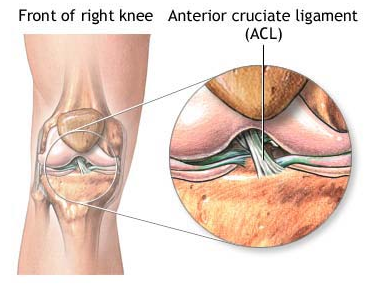
\includegraphics[width=3in]{images/acl_anatomy.bmp}
  \end{center}
  \caption{Knee anatomy and location of ACL}
  \label{fig:knee_anatomy}
\end{figure}

\subsection{Knee Flexion Angles}
ACL is responsible for resisting anterior translation and medial rotation of the tibia, in relation to the femur. This resistance is crucial for controlling the forward movement and twisting of the knee. Major cause of ACL injury is small knee flexion angle along with medial rotation. The knee flexion angle is the angle between the femur and the tibia. The medial rotation is the internal rotation of the knee towards the midline axis of the human body. As a result, these angles are an important indicator for the injury.

\subsection{Asymmetric distributed forces}
Another common reason for the ACL injury is due to asymmetric distributed forces acting on the joint. As these forces are not equally distributed, the resultant force direction does not pass through the vertical axis at the center of the leg. This resultant force causes anterior translation and medial rotation. Once the forces exceed the resistance offered by the ACL,  the ACL ruptures due to excessive strain (TODO cite GRIFFIN et al). Now, these forces are caused due to sudden movements such as changing directions or landing from a jump, which are most common in sports (TODO cite GRIFFIN et al). These decelerations generally happen as fast as 50ms (TODO cite some paper), and therefore, ekwip needs to be able to measure the deceleration as fast as 10s of milliseconds. The decelerations can then be related to the forces to provide a more complete analysis for risk calculations.

\section{Related Work}
\label{sec:related_work}
Related work for this project is divided among three fields: algorithms for ACL injury detection (Section 2.1), knee brace effectiveness/performance hindrance (Section 2.2), and Smart Materials (Section 2.3). ACL injury detection covers previous research in minimizing the testing required to detect whether an athlete is at risk of suffering an ACL injury. Knee brace effectiveness/performance hindrance deals mainly with studies of the extent to which a Functional Knee Brace and a Prophylactic Knee Brace play in the ability for an athlete to perform on the field. Finally, Smart Materials concern the reach for this project and the possibility of actually preventing the ACL injuries from occurring on the field.

\subsection{ACL Injury Detection} Prior research in ACL Injury Detection have shown that techniques exist that accurately capture and analyze various measures relating to the knee to determine the probability of ACL injuries \cite{smedicine}. Using such metrics as knee valgus motion, knee flexion rotation of motion, and body mass, researchers were able to come up with a way to determine knee abduction moments (KAM), which are used to identify whether or not an athlete is at high risk for an ACL injury, with a sensitivity of 77\% and specificity of 71\% \cite{smedicine}\cite{Bahr01062005}. 

\subsection{Knee Brace Effectiveness/ Performance Hindrance} Prior research in using Functional or Prophylactic knee braces out in the field useful but results on the potential hindrance of using these kinds of braces were inconclusive \cite{Myer01042011}. Knee braces, especially Functional Knee Braces (FKB), which are more mechanical in nature and thus more obtrusive, are shown to provide “20-30\% greater knee ligament protection”. This suggests that FKBs have an impact in reducing the severity of knee injuries. More testing needs to be done to see whether or not FKBs will actually hinder the performance of an athlete. Another important factor of the effectiveness of knee braces is in rehabilitation, where a combination of exercises and brace use can speed up recovery \cite{hewett2010acl} .

\subsection{Smart Materials} Prior research in the use of Electro-rheological fluids (ERF) show that these material reacts quickly when presented with an electric field, have a high yield stress, and are very lightweight and easily molded \cite{smaterials}. ERF can quickly change viscosities, which make it an excellent material to use in the project. Due to the very nature of ERF’s fast response and simple interface, using it in a light, functional knee brace would allow lead to an easy implementation of the preventative nature of the project.

\section{Project Proposal}
\label{sec:project_proposal}
This project focuses on the research and development of eKwip, an electronic knee wrap for injury prediction and prevention, for both healthy athletes as well as patients recovered from an ACL injury. Unlike traditional mechanical knee braces, eKwip is unobtrusive and flexible. It is able to adapt to and learn the pattern of movements of its wearer, closely monitor the performance of his or her knee, predict when an injury is imminent and reduce the impact of the injury. Through eKwip, the wearer or physical therapist is able to monitor the performance of the knee and assess the risk of injury in the future through a simple user interface. This can allow both healthy athletes to reduce the risk of injury, as well as allow injured patients to monitor their risk of reinjury over time. eKwip also provides an easy way for physical therapist to observe their patients and judge whether they are fit to return to sports.


\subsection{Anticipated Approach}
\label{subsec:approach}
The project is split into three sections - measurement, prediction and prevention. The project will focus on achieving all the goals in measurement and prediction, while attempting to tackle prevention if time permits.

\subsubsection{Phase 1 - Measurement}
This part of the project focuses on the research and implementation of the knee wrap to collect measurements and monitor movements in the knee. The wrap should be able to store the collected data and relay it through a user friendly interface. At the end of this phase, a basic functioning prototype should be created.

The first part of this phase includes the research and understanding of ACL injuries in order to decide which measurements to take. In order to better understand the factors that contribute to an ACL injury - the different angles, forces and orientation of the knee, doctors and experts in field will be consulted. The secondary purpose of meeting with experts in the field is to identify the group of people with the highest risk of injury, which provides a better focus for the project. As it currently stands, it seems that female athletes are at higher risk of sporting ACL injuries - a rate of 2 to 10 times more likely to sustain ACL injuries compared to male athletes playing the same landing and cutting sports \cite{smaterials}. The potential value of this knee wrap can also be estimated by determining the benefits to different fiends in the current market, such as rehabilitation and sports health.

Once the necessary measurements needed to predict an injury is determined, a prototype of the wrap will be built. The basic prototype will consist of a simple elastic knee wrap, an mbed microcontroller (LPC1768) and sensors (Pololu UM6-LT Orientation Sensor). The microcontroller will be programmed and connected to the sensors and the sensors will be calibrated to give precise measurements. The prototype wrap will be worn and tested and measurements collected. The range of the different measurements according to the constraints of the knee will be observed which will allow further calibration of the sensors. Different sampling rates will be tested and the one with the highest precision to memory cost ratio will be used.

The prototype wrap should also be able to store the measurements in its internal memory and able to output to a computer via USB or ethernet connection. A simple user interface will be built in order to give some sort of visualization of the knee movements over the time frame as well as the different measurements collected.

\subsubsection{Phase 2 - Prediction}
This part of the project focuses mainly on the prediction aspect of eKwip. The goals of this phase includes implementation of an algorithm to determine the risk of ACL injury given the measurements. A risk index will be compiled to indicate the knee performance of wearer and the risk of injury. Since different people have different ranges of tolerable movements, it is necessary for the wrap to be flexible and adaptive, in order to determine the risk of injury for each individual. Secondly, the prototype at the end of this stage should be able to predict the risk of injury in real time, with precision up to tens of milliseconds. This allows possible real time prevention of the injury once the prevention mechanism is developed in phase 3. Lastly, the knee wrap should be able to communicate with the server wirelessly to transmit data of his or her movements to allow the wearer to be monitored in real time.

The research portion of this phase includes collection of data, determining the risk of injury given a set of movements and creating a risk index. This requires further meetings with experts in the field to better understand the biomechanics of the knee and limits of the ACL given a set of measurements, such as position, orientation, speed and load. Since testing on human subjects is not a possibility, research in this phase is very important to determine the risk of injury and to come up with the risk index.

Once the risk index has been determined, the functionality of the prototype knee wrap can then be extended to include real time prediction of injury. This is done by predicting the future position, orientation and load on the knee based on current measurements. In order to achieve real time prediction, the sampling rate of the measurements will be increased in order to give a more precise reading. However, due to the memory limitations, the measurements from this increased sampling rate will not be stored to memory. Furthermore, a learning algorithm will be implemented in order for the knee wrap to adjust to the different range of movements of each individual in order to provide a personalized risk index and injury prediction. Based on the complexity and processing power required for this learning algorithm, the algorithm will either reside on the microcontroller or on the server side, syncing only the necessary information to and from the knee wrap when it is connected. With the latter implementation, the server should have a database to keep track of the data for each wearer. Lastly, a wireless module (WIFI or Bluetooth) will be added to eKwip to allow it to wirelessly connect to the server whenever it is in range. This reduces the trouble of having to physically remove and connect the wrap to a computer via a cord.

\subsubsection{Phase 3 - Prevention}
The last part of the project, focusing on injury prevention, will be completed if time permits. In this phase, a prevention mechanism will be designed and implemented into eKwip. The goal of the prevention mechanism is to reduce the impact of injury and possibly preventing the injury completely.

The prevention mechanism needs to be unobtrusive when not engaged to allow full movements of the knee, while preventing the knee from bending past at certain angles when engaged. A possible approach is the use of smart materials, in particular electrorheological fluids and magnetorheological fluids. These material will act as a fluid normally, while changing its viscosity and transforming into a solid state when either an electric field or magnetic field is applied. If these materials can be integrated into eKwip, it would be placed on the outside of the leg parallel to the knee to lessen the impact of the valgus force, which often contributes to an ACL injury, and placed vertically along the kneecap to directly protect the ACL. Once eKwip is able to predict when an injury is imminent, it can trigger an electric or magnetic field to change the viscosity of the smart materials in stages to absorb the impact and hopefully prevent the injury. Areas of further research involves discovering other possible approaches to eKwip’s prevention mechanism, analyzing the side effects of such prevention mechanisms, and testing their effectiveness. 



\subsection{Technical Challenges}
\label{subsec:tech_challenges}
There are several technical and non-technical challenges expected from this project. The first major challenge includes determining the variables to be measured from the knee in order to effectively predict the risk of injury. This includes a lot of experimenting, researching and consulting experts in field to correctly identify the features that best indicates an imminent ACL injury. Since there is a trade off between measuring and collecting as much information as possible, and the storage cost and processing power of the microcontroller, only the critical variables should be identified and used in the prediction process. Given the set of necessary measurements, such as relative angle, speed and orientation of knee, the placement of the sensors need to be designed to be as unobtrusive to the wearer as possible while still able to collect precise and accurate measurements from the knee. With this set of measurements defined, the knee can be effectively modelled. Currently, aside from the knee valgus motion, knee flexion range of motion, and body mass, there may be more measurable factors directly contributing to ACL injury that have yet to be determined, and thus will be a huge challenge for this project \cite{Myer01042011}.

The second major challenge involves determining the risk of injury for each individual. Since the different wearers are likely going to have different range of tolerable movements based on their fitness, gender, age and training, it is necessary for the wrap to be adaptive and flexible. Thus, the wrap needs to be able to use the collected data to make adjustments to its prediction algorithm through reinforcement learning. The challenge, however, is that the knee wrap will mostly be exposed to healthy movements in which an injury is not about to occur. It lacks the data for when an injury is occurring and therefore negative feedback is not possible. Therefore, the learning algorithm needs to be designed to be able to learn the range of movements of the wearer with only the limited dataset available.

Another major challenge is to come up with a risk index given the collection of data. Since the goal of the risk index is for it to eventually become a universal way to estimate the risk of ACL injury, it is necessary for the index to be as accurate as possible, and customized to the physique of the wearer. The construction of such an index is very complicated as it needs to take into account of the physique of the individual wearing the wrap, combined with the index currently used in rehabilitation, and assessments used to judge whether athletes are ready to return to sports after an injury \cite{Sinkjar1991209}. Although this is an ambitious task, and haven’t been accomplished before, coming up with a universal risk index to assess the possibility of ACL injury and reinjury is very useful for monitoring the performance of athletes or injured patients.

A major technical challenge to this project is to be able to collect measurements at a high enough frequency to predict and prevent the ACL injury in real time. Depending on the frequency of measurements needed to allow enough time for the microcontroller to calculate and react, some parts of the code may have to be written in a low level language, such as assembly, to decrease the processing time. The first challenge here is to identify these bottlenecks in the code and the subsequent challenge is to optimize those sections to run as fast as possible without sacrificing precision and accuracy of the injury prediction. This can allow eKwip to detect and predict ACL injuries in real time and react as fast as tens of milliseconds.

The project also presents some design challenges. The eKwip wrap should be designed as comfortable and unobtrusive as possible to not hinder the movements of athletes and patients until an injury is imminent. The wrap should be light and flexible to encourage athletes to wear it even if they have a healthy knee. This requires careful choice of microcontrollers, sensors and other components in the wrap, as well as the positioning of such components. Ultimately, eKwip should be designed to be flexible to fit athletes and patients of different body types.

Lastly, the project also presents some material and mechanical challenges. In order to prevent the ACL injury, the wrap has to be equipped with a prevention mechanism capable of absorbing huge forces and supporting the weight of the wearer. A possible approach, as mentioned in 3.1.3, is the use of smart materials that is capable of changing viscosity. However, in order to create substantial support for the knee, a large electric field or magnetic field has to be used. Depending on the size of field, this approach may be impossible for a portable wrap like eKwip. This will be explored further if time permits. 

\subsection{Evaluation Criteria}
\label{subsec:eval_criteria}
In order to determine whether eKwip performs as intended, it is necessary to evaluate the knee wrap after the prototype is built and compare its performance with the current knee wraps. Since there are currently no knee wraps on the market that accomplishes all of what eKwip sets out to do, eKwip's different functionalities are to be compared with the different equivalent products and services out there.

To determine the effectiveness and accuracy of the injury prediction and risk assessment part of eKwip, one can compare it to other commonly used knee stability assessments in rehabilitation centers , such as the use of electromyographic measurements from muscles acting on the knee \cite{Sinkjar1991209}. Patients who suffered ACL injury can wear the eKwip knee wrap and their performance on those knee stability assessments can be compared to the risk prediction rating generated by eKwip to see if eKwip correctly identifies the health of the injured knee. If a correlation is found, then eKwip is able to successfully and reliably measure the health of a person’s knee without needing him or her to undergo a set of assessments under supervision. 

Other than performing correlation analysis on eKwip, one can also judge the quality and effectiveness of eKwip through the opinions of experts in the field. Doctors and physical therapists can use eKwip to monitor their patients and determine whether eKwip is easier and as accurate at monitoring patients over the traditional ways of monitoring. However, this evaluation criteria is more subjective and should not be weighted as much as the objective criteria suggested earlier.

On the other hand, the effectiveness of the prevention mechanism of eKwip can be assessed and compared against the traditional mechanical braces. Patients who have recovered from ACL injuries will choose to wear either a mechanical brace, eKwip, or no braces at all. The reinjury rate across the three groups can then be collected through a survey and the effectiveness of each method can be successfully compared.


\section{Research Timeline}
\label{sec:research_timeline}
The project timeline is split into the following sections - already completed, prior to thanksgiving, prior to Christmas, completion and if time permits.

\begin{enumerate}
    \item Already completed:
    \begin{itemize*}
        \item Ordering of materials required for first prototype
        \item Speak with experts in field to find out possible causes of ACL tear
        \item Speak with doctors to find out the benefit of such a product to the field
    \end{itemize*}
    \item Prior-to thanksgiving
    \begin{itemize*}
        \item Prototype built
        \item Preliminary data collected
    \end{itemize*}
    \item Prior-to christmas
    \begin{itemize*}
        \item Phase 1 completed
        \item Tweaking of sensors and measurements on prototype
        \item Allow data to be stored on microcontroller
        \item Capable of displaying data collected in a user friendly interface.
    \end{itemize*}
    \item Completion tasks
    \begin{itemize*}
        \item Phase 2 completed
        \item Speak with experts in field to determine risk index
        \item Conduct more testing to improve accuracy of measurements
        \item Real time prediction of injury
        \item Streaming of data from wrap to server
        \end{itemize*}
    \item If there's time
    \begin{itemize*}
        \item Phase 3 completed
        \item Research material needed for injury prevention mechanism
        \item Integrate material with eKwip
        \item Connect the prevention mechanism to the prediction algorithm
    \end{itemize*}
\end{enumerate}



% We next move onto the bibliography.
\bibliographystyle{plain} % Please do not change the bib-style
\bibliography{sections/references}  % Just the *.BIB filename

\end{document} 

